%% indica que é uma apresentação de slides (beame)
\documentclass{beamer}

%%------------------------------------------------------------------------------%%
%% padrão de caracteres e língua
\usepackage[utf8x]{inputenc}
\usepackage[brazil]{babel}

%%------------------------------------------------------------------------------%%
%% nao sei bem pra q iso xD
\usepackage{graphicx}

%%------------------------------------------------------------------------------%%
%% tema, estilo dos slides...
\usetheme{Copenhagen}
\usecolortheme{whale}
%% site onde tem todos os disponíveis:
%%   http://www.hartwork.org/beamer-theme-matrix/

%%------------------------------------------------------------------------------%%
%% informações utilizadas pelo pacote (no caso Copenhagen) para
%% montar o 'slide padrão', com informações dos autores na base
%% bem como para montar um slide predefinido chamado 'title page'

%% O [Título Resumido] aparece em todos os slides bem pequeno
%% O {Título Completo} aparece apenas no slide 'title page'
%%   Se for um título composto, escreve-se \\ para inserir uma quebra de linha
%%   pulei linhas para ficar mais organizados, mas ele ignora e considera apenas o \\

\title[CRINTER]{CRINTER: Criador de Interfaces}

\author[Anderson, Ane, Lia, Lucélia, Silvia Oliveira]
       {Anderson Pimentel \\ Ane de Souza \\  Lia Martins \\
       Lucélia Mota \\ Silvia Oliveira}

\institute[UEA]{Universidade do Estado do Amazonas-UEA\\Escola Superior de Tecnologia-EST}

\date{}


\begin{document}

%% esse slide é montado com as informações já passadas acima (no cabeçalho)
%% é o primeiro slide que aparece, pois é a primeira definição de frame após o
%% início do documento
%% ===================SLIDE 1==================== %%
\frame{\titlepage}

%% Esse slide é criado com informações de \section que podemos definir se quisermos
%% mais a frente ficará bem claro como isso funciona, pule esse slide nesse momento
%% ===================SLIDE 2==================== %%
\begin{frame}
  \frametitle{Descrição}
  Um software para criar interface de forma ágil para auxiliar desenvolvedores na interação com o cliente. Pois a interface é um ponto crítico para aceitação ou não do software.
  
\end{frame}


\begin{frame}
  \frametitle{Modelo da Interface}

  \begin{figure}[htp]
        \centering
        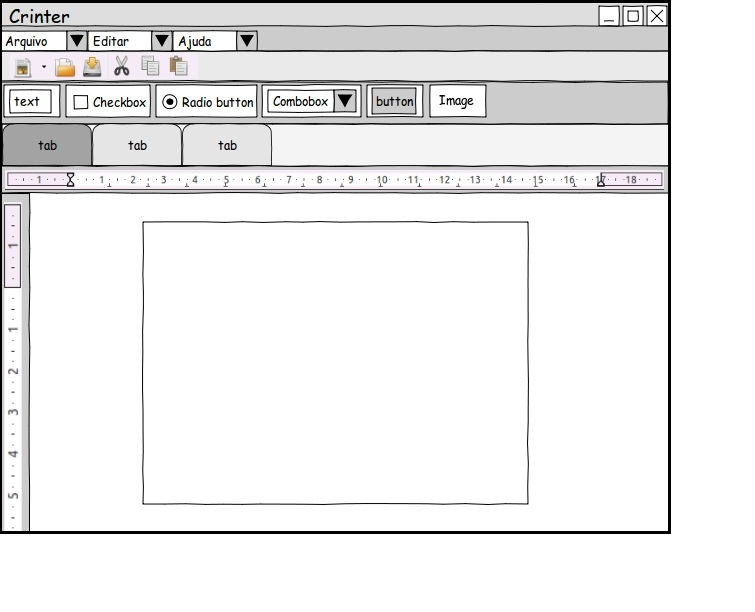
\includegraphics[width=0.7\textwidth]{InterfaceCrinter}\\
      \end{figure}

	\end{frame}
	
	
\begin{frame}
  \frametitle{Requisitos Funcionais}
\begin{itemize}

\item O software deve permitir o usuário criar projeto.
\item O software deve permitir o usuário salvar  o projeto.
\item O software deve permitir o usuário abrir o projeto.
\item O software deve permitir o usuário criar  nova página.
\item O software deve permitir salvar página.
\item O  software deve permitir a visualização das páginas criadas em abas.
\item O software deve permitir a visualização da página.
\item O software deve permitir o usuário  criar o layout da página.
\item O software deve permitir o usuário  inserir painel.

\end{itemize}

	\end{frame}
	
	
\begin{frame}
  \frametitle{Requisitos Funcionais}
\begin{itemize}


\item O software deve permitir o usuário redimensionar  painel.
\item  O software deve permitir o usuário alterar  a cor do painel.
\item  O software deve permitir o usuário  mover painel.
\item  O software deve permitir o usuário  inserir label.
\item  O software deve permitir o usuário  redimensionar label.
\item O software deve permitir o usuário  editar label.
\item  O software deve permitir o usuário  alterar fonte (cor, tamanho, estilo) do label.
\item  O software deve permitir o usuário  mover label.
\item  O software deve permitir o usuário  inserir caixa de texto.
\item  O software deve permitir o usuário  redimensionar caixa de texto.

\end{itemize}

	\end{frame}

\begin{frame}
  \frametitle{Requisitos Funcionais}
\begin{itemize}

\item  O software deve permitir o usuário  editar caixa de texto.
\item   O software deve permitir o usuário  alterar fonte (cor, tamanho, estilo) da caixa de \item  texto.
\item   O software deve permitir o usuário  mover caixa de texto.
\item   O software deve permitir o usuário  inserir botões radiais.
\item   O software deve permitir o usuário  alterar o nome do botão radial.
\item   O software deve permitir o usuário  mover os botões radiais.
\item  O software deve permitir o usuário  redimensionar o botão radial.



\end{itemize}

	\end{frame}

\begin{frame}
  \frametitle{Requisitos Funcionais}
\begin{itemize}

\item   O software deve permitir o usuário  inserir caixa de seleção combobox.
\item   O software deve permitir o usuário  alterar o nome do combobox.
\item   O software deve permitir o usuário  redimensionar combobox.
\item   O software deve permitir o usuário  mover o combobox.
\item  O software deve permitir o usuário  inserir área de texto.
\item O software deve permitir o usuário  alterar fonte (cor, tamanho, estilo) da área de texto.
\item  O software deve permitir o usuário  redimensionar área de texto
\item  O software deve permitir o usuário  mover a área de texto.


\end{itemize}

	\end{frame}

\begin{frame}
  \frametitle{Requisitos Funcionais}
\begin{itemize}

\item  O software deve permitir o usuário  remover qualquer elemento inserido na página.
\item  O software deve permitir o usuário inserir botões.
\item  O software deve permitir o usuário redimensionar botão.
\item  O software deve permitir o usuário mover botão.
\item  O software deve permitir o usuário alterar nome do botão. 
\item  O software deve permitir o usuário importar imagem.
\item  O software deve permitir o usuário exportar para PNG.
\item   O software deve  permitir o usuário ver uma régua.
\item   O software deve salvar automaticamente as alterações de uma página já salva. 

\end{itemize}

	\end{frame}
	


\begin{frame}
  \frametitle{Requisitos Não-Funcionais}
  
\begin{itemize}


\item  O software  deverá ser criado no Eclipse Helios.
\item   O software  deverá ser modelado seguindo regras da UML 2.0.
\item   O software  deverá usar Junit para testes.
\item   O software  deverá usar o Git para controle de versões.
\item   O software  deverá ser modelado em diagramas e casos de uso no Astah ou Umbrello.
\item   O software  deverá ser documentado em Latex.
\item   O  software deverá utilizar o Ant.

\end{itemize}
  

	\end{frame}
	
\end{document}
